\documentclass[11pt]{article}
\usepackage[margin = 1in]{geometry}
\usepackage{amsmath}
\usepackage{amssymb}
\usepackage{amsthm}
\usepackage{graphicx}
\usepackage{enumitem}
\usepackage{url}
\usepackage[parfill]{parskip}
\usepackage{listings}
\usepackage{caption}
\usepackage{subcaption}
\usepackage[utf8]{inputenc}
\usepackage{xcolor}
\definecolor{codegreen}{rgb}{0,0.6,0}
\definecolor{codegray}{rgb}{0.5,0.5,0.5}
\definecolor{codepurple}{rgb}{0.58,0,0.82}
\definecolor{backcolour}{rgb}{0.95,0.95,0.92}
\lstdefinestyle{mystyle}{
	backgroundcolor=\color{backcolour},   
	commentstyle=\color{codegreen},
	keywordstyle=\color{magenta},
	numberstyle=\tiny\color{codegray},
	stringstyle=\color{codepurple},
	basicstyle=\ttfamily\footnotesize,
	breakatwhitespace=false,         
	breaklines=true,                 
	captionpos=b,                    
	keepspaces=true,                 
	numbers=left,                    
	numbersep=5pt,                  
	showspaces=false,                
	showstringspaces=false,
	showtabs=false,                  
	tabsize=2
}
\lstset{style=mystyle}
\newcommand{\skipline}{\vspace{\baselineskip}}
\newcommand{\spacer}{\noalign{\medskip}}
\newcommand{~}{\sim}
\newcommand{\approches}{\rightarrow}
\newcommand{\qarrow}{\quad \rightarrow \quad}
\newcommand{\qqarrow}{\qquad \rightarrow \qquad}
\newcommand{\qqtext}[1]{\qquad \text{ #1 } \qquad}
\newcommand{\pard}[2]{\frac{\partial #1}{\partial #2}}
\newcommand{\answer}[1]{\textbf{\boldmath #1}}
\newenvironment{problem}[1]{\textbf{Problem #1: }}{\newpage}

\begin{document}
	
	\begin{center}
		\textbf{Exam 1} \\
		\textbf{Partial Differential Equations} \\
		\textbf{Math 531} \\
		\textbf{Stephen Giang RedID: 823184070} \\
		\skipline \skipline
	\end{center}

	I, \underline{Stephen Giang} , pledge that this exam is completely my
	own work, and that I did not take, borrow or steal work from any other person, and that I did
	not allow any other person to use, have, borrow or steal portions of my work. I understand that
	if I violate this honesty pledge, I am subject to disciplinary action pursuant to the appropriate
	sections of the San Diego State University Policies.

	\skipline
	\begin{problem}{1}
		\begin{enumerate}[label = (\alph*)]
			\item Find the eigenvalues and eigenfunctions for the Sturm-Liouville problem
			\[\phi'' + \lambda \phi = 0, \qquad 0 < x < 4\]
			\[\text{with B.C.'s } \quad \phi(0) = 0 \quad\text{ and }\quad 2\phi(4) + \phi'(4) = 0.\]
			\\ 
			For the Sturm-Liouville problem, we consider the three cases of $\lambda$:
			\begin{enumerate}[label = (\alph*)]
				\item ($\lambda = 0$): Notice the following:
				\[\phi'' = 0 \qquad \phi' = c_1 \qquad \phi = c_1x + c_2\]
				We can now use our boundary conditions, and we get:
				\[\phi(0) = 0 = c_2 \qqarrow \phi(x) = c_1x\]
				\[2\phi(4) + \phi'(4) = 2(c_1(4)) + c_1 = 9c_1 = 0 \qqarrow c_1 = 0\]
				Thus, we get the following trivial solution:
				\[\boldsymbol{\phi(x) = 0}\]
				\item ($\lambda < 0$): Notice the following:
				\[\phi'' - |\lambda|\phi = 0\]
				Using the characteristic equation, we get:
				\[\phi(x) = c_1\cosh(\sqrt{|\lambda|}x) + c_2\sinh(\sqrt{|\lambda|}x) \qquad \phi'(x) = c_1\sqrt{|\lambda|}\sinh(\sqrt{|\lambda|}x) + c_2\sqrt{|\lambda|}\cosh(\sqrt{|\lambda|}x) \]
				We can now use our boundary conditions, and we get:
				\[\phi(0) = c_1 = 0 \qquad \phi(x) = c_2\sinh(\sqrt{|\lambda|}x)\]
				\[2\phi(4) + \phi'(4) = 2c_2\sinh(4\sqrt{|\lambda|}) + c_2\sqrt{|\lambda|}\cosh(4\sqrt{|\lambda|}) = 0\]
				\[c_2\left(2\sinh(4\sqrt{|\lambda|}) + \sqrt{|\lambda|}\cosh(4\sqrt{|\lambda|})\right) = 0\]
				\[2\sinh(4\sqrt{|\lambda|}) + \sqrt{|\lambda|}\cosh(4\sqrt{|\lambda|}) = 0 \qqarrow \tanh(4\sqrt{|\lambda|}) = \frac{-\sqrt{|\lambda|}}{2} \]
				Assuming $c_2 = 0$ will give us the trivial solution.  Assuming $c_2 \not= 0$, we get the only eigenvalue and eigenfunction to be:
				\[\boldsymbol{\lambda = 0 \qqarrow \phi(x) = 0}\]
				\item ($\lambda > 0$): Notice the following:
				\[\phi'' + \lambda\phi = 0\]
				Using the characteristic equation, we get:
				\[\phi(x) = c_1\cos(\sqrt{\lambda}x) + c_2\sin(\sqrt{\lambda}x) \qquad \phi'(x) = -c_1\sqrt{\lambda}\sin(\sqrt{\lambda}x) + c_2\sqrt{\lambda}\cos(\sqrt{\lambda}x)  \]
				We can now use our boundary conditions, and we get:
				\[\phi(0) = c_1 = 0 \qqarrow \phi(x) = c_2\sin(\sqrt{\lambda}x)\]
				\begin{align*}
					2\phi(4) + \phi'(4) = 2c_2\sin(4\sqrt{\lambda}) + c_2\sqrt{\lambda}\cos(4\sqrt{\lambda}) &= 0 \\
					c_2\left(2\sin(4\sqrt{\lambda}) + \sqrt{\lambda}\cos(4\sqrt{\lambda})\right) &= 0
				\end{align*}
				\begin{enumerate}[label = (\roman*)]
					\item $(c_2 = 0)$:
					\[\phi(x) = 0\]
					Thus we get the following trivial solution:
					\item $2\sin(4\sqrt{\lambda}) + \sqrt{\lambda}\cos(4\sqrt{\lambda}) = 0$:
					\[\tan(4\sqrt{\lambda}) = -\frac{4\sqrt{\lambda}}{2(4)}\]
					Assuming $c_2 = 0$ will give us the trivial solution.  Assuming $c_2 \not= 0$, we can use software such as Matlab to approximate the eigenvalues and also get the corresponding eigenfunction:
					\[\boldsymbol{\lambda_n \approx \left( \frac{(n - \frac{1}{2})\pi}{4}\right) ^2 \qqarrow \phi_n(x) = c_2\sin\left(\sqrt{\lambda} x \right)}\]
				\end{enumerate}
			\end{enumerate}
			\item  Use the eigenfunctions from Part a to represent the function
			\[f(x) = \begin{cases}
				5, \qquad & 0 < x < 2, \\ 0, \qquad & 2 \leq x < 4
			\end{cases}\]
			and find the generalized Fourier coefficients.
			\\ \\
			Applying the function given, we get:
			\[\phi(x) = f(x) = \sum_{n=1}^{\infty} B_n\sin\left(\sqrt{\lambda_n}x \right)\]
			Using the orthogonality of sines, we get:
			\begin{align*}
				B_n &= \frac{2}{4}\int_{0}^{4} f(x)\sin\left(\sqrt{\lambda_n}x \right) \\
				&= \frac{1}{2}\left[\int_{0}^{2} 5\sin\left(\sqrt{\lambda_n}x \right) + \int_{2}^{4} 0\sin\left(\sqrt{\lambda_n}x \right)\right] \\
				&= -\frac{5\sqrt{\lambda_n}}{2}\cos\left(\sqrt{\lambda_n}x\right)\bigg|_0^2 \\
				&= -\frac{5\sqrt{\lambda_n}}{2}\left(\cos\left(2\sqrt{\lambda_n}\right) - 1\right)
			\end{align*}
			\newpage
			\item What does the Fourier series converge to at $x = 1$? at $x = 2$? at $x = 3$? at $x = -1$? Does
			this Fourier series produce a periodic extension for all $x$? Explain.
			\\ \\
			At $x = 1$, the series will converge to $f(x) = 5$.  At $x = 2$, the series will converge to $f(x) = 5/2$. At $x = 3$, the series will converge to $f(x) = 0$. At $x = -1$, the series will converge to $f(x) = 0$.  The Fourier series will produce a periodic extension for all $x$, as it has a period of $x = L = 4$.
			\item Use the computer to find the numerical values of the first 50 eigenvalues. (Only write the
			values for $\lambda_1, \lambda_2, \lambda_5, \lambda_{10}, \lambda_{25}, \text{ and } \lambda_{50}$.) Graphically, show $f(x)$ and the approximation using 50 terms in the Fourier series for $x \in [0, 4]$ and $x \in [-4, 8]$. What is the absolute error between your 50 term Fourier series and the value of $f(x)$ at $x = 0.05, x = 1, x = 2.5, \text{ and } x = 3.75$. Find the maximum actual error between the 50 term approximation and the actual function.
			(The maximum error is for the Gibbs's phenomenon and not the obvious error caused by the
			jump discontinuity.) Give both the $x_{max} \in (0, 4)$ value and the Fourier series value at $x_{max}$ for
			this maximum error.
			\\ \\
			The following are the requested eigenvalues:
			\[\lambda_1 = 0.4916, \qquad \lambda_2 = 2.0071, \qquad \lambda_5 = 13.3908 \]
			\[\lambda_{10} = 45.5344, \qquad \lambda_{25} = 341.6510, \qquad \lambda_{50} = 1451.9850\]
			The following are the absolute errors:
			\[x = 0.05 : \text{error = } 1981.2933 \qquad x = 1 : \text{error = } 172.5518 \]
			\[x = 2.5 : \text{error = } 63.8272	\qquad x = 3.75 : \text{error = } 93.9407\]
			Notice the following values of the maximum error:
			\[x = 0.0540 : \text{error = }  1999.5942\]
			\begin{figure}[h!]
				\centering
				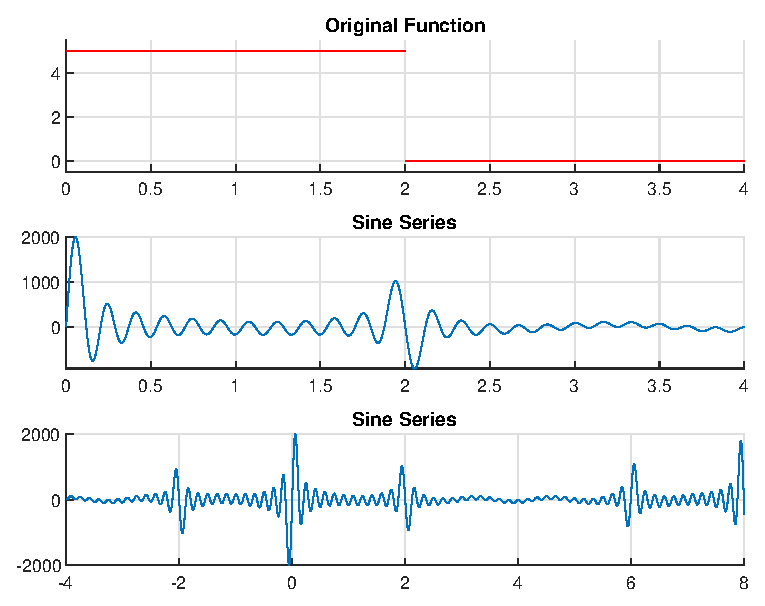
\includegraphics[width=.55\linewidth]{./Code/Prob1d}
			\end{figure}
			\newpage
			\lstinputlisting[language=Matlab]{./Code/Prob1d.m}
		\end{enumerate}
	\end{problem}

	\begin{problem}{2}
		Consider the non-homogeneous heat equation given by:
		\[\frac{1}{k} \pard{u}{t} = \pard{^2u}{x^2} - \gamma^2(u - T), \qquad 0 < x < L, \qquad  t > 0.\]
		With boundary conditions and initial condition:
		\[u(0,t) = T_0, \qquad u(L,t) = T_1, \quad\text{ and }\quad u(x,0) = 0\]
		Give a physical interpretation of the partial differential equation, its parameters, and its boundary and initial conditions. Solve the steady state problem.
		\\ \\
		This partial differential equation represents heat in a one-dimensional rod. The term $ - \gamma^2(u - T)$ represents a heat sink, such that heat is being lost over time.  The term $k$ represents the thermal conductivity. The boundary conditions represent the temperature at different endpoints of the rod.  The initial condition represents the amount of heat energy in the rod at time $t = 0$.
		\\ \\
		Notice we can let the following be true because of the fact that this is a steady state problem:
		\[\frac{1}{k} \pard{u}{t} = \pard{^2u}{x^2} - \gamma^2(u - T) = 0 \qqarrow \frac{d^2u}{dx^2} - \gamma^2u = -\gamma^2T\]
		This is simply an ODE problem now with the following general and particular solutions:
		\[u_h(x) = c_1\cosh(\gamma x) + c_2\sinh(\gamma x) \qquad u_p(x) = T\]
		Thus the solution to this steady state problem is the following:
		\[u(x) = u_h + u_p = c_1\cosh(\gamma x) + c_2\sinh(\gamma x) + T\]
		Using our given boundary conditions, we get the following coefficients:
		\[u(0) = c_1 + T = T_0 \qarrow c_1 = T_0 - T\]
		\[u(L) = (T_0 - T)\cosh(\gamma L) + c_2\sinh(\gamma L) + T = T_1 \qarrow c_2 = \frac{T_1 - T - (T_0 - T)\cosh(\gamma L)}{\sinh(\gamma L)}\]
		So we get the final solution to be:
		\[\boldsymbol{u(x) = (T_0 - T)\cosh(\gamma x) + \frac{T_1 - T - (T_0 - T)\cosh(\gamma L)}{\sinh(\gamma L)}\sinh(\gamma x) + T}\]
	\end{problem}

	\begin{problem}{3}
		Consider the heat equation given by:
		\[\pard{u}{t} = k\nabla^2u, \qquad 0 < x < 2, \qquad 0 < y < 3, \qquad t > 0.\]
		With boundary conditions:
		\[\pard{u}{x}(0,y,t) = A(3-y), \qquad \pard{u}{x}(2,y,t) = y^2, \qquad \pard{u}{y}(x,0,t) = 0, \qquad \text{and} \qquad \pard{u}{y}(x,3,t) = 0,\]
		and initial condition:
		\[u(x,y,0) = x(3-y).\]
		Find the condition on $A$ ($A$ constant) that allows the steady state problem to be solvable on
		the rectangular domain. Solve the steady state problem. 
		\\ \\
		For the steady state problem to be solvable on the rectangular domain, we have to let $A = 0$:
		\[\pard{^2u}{x^2} + \pard{^2u}{y^2} = 0 \qquad 0 \leq x \leq 2, \qquad 0 \leq y \leq 3\]
		with 
		\[u(x,y) = \phi(y)h(x), \qquad \phi'(0) = 0, \quad \phi'(3) = 0, \quad h'(0) = 0\]
		Taking Laplace's Equation, we get the following:
		\[\phi''(y)h(x) + \phi(y)h(x)'' = 0\]
		\[\frac{\phi''(y)}{\phi(y)} = -\frac{h''(x)}{h(x)} = -\lambda\]
		From this, we get the following:
		\[\phi'' + \lambda \phi = 0, \qquad h'' - \lambda h = 0\]
		\newpage
		From this, we can see this is an eigenvalue problem:
		\begin{enumerate}[label = (\alph*)]
			\item $(\lambda = 0)$:
			\[\phi'' = 0 \qqarrow \phi' = c_1 \qqarrow \phi = c_1y + c_2\]
			\[h'' = 0 \qqarrow h' = d_1 \qqarrow h = d_1x + d_2\]
			Substituting in our BC's, we get:
			\[\phi'(0) = \phi'(3) = c_1 = 0 \qqarrow \phi(y) = c_2\]
			So now we have our first eigenfunction:
			\[\phi(y) = c_2 \text{ with } \lambda = 0\]
			Now we can solve for $h(x)$:
			\[h'(0) = d_1 = 0 \qarrow h(x) = d_2 \]
			From here, we get the following:
			\[u(x,y) = c_2d_2\]
			Now we can simply set the following and get the first product solution:
			\[\boldsymbol{u_0(x,y,t) = A_0}\]
			\item $(\lambda < 0)$:
			\[\phi'' - |\lambda|\phi = 0\]
			Using the characteristic equation, we get:
			\[\phi(y) = c_1\cosh(\sqrt{|\lambda|}y) + c_2\sinh(\sqrt{|\lambda|}y) \qquad \phi'(y) = c_1\sqrt{|\lambda|}\sinh(\sqrt{|\lambda|}y) + c_2\sqrt{|\lambda|}\cosh(\sqrt{|\lambda|}y) \]
			Using the BC's, we get:
			\[\phi'(0) = c_2\sqrt{|\lambda|} = 0 \qarrow \sqrt{|\lambda|} > 0 \qarrow c_2 = 0\]
			\[\phi'(3) = c_1\sqrt{|\lambda|}\sinh(3\sqrt{|\lambda|}) = 0 \qarrow \sqrt{|\lambda|}\sinh(3\sqrt{|\lambda|}) \not = 0 \qarrow c_1 = 0\]
			\[\phi(y) = 0\]
			Thus we get the following trivial solution:
			\[\boldsymbol{u(x,y,t) = 0}\]
			\item $(\lambda > 0)$:
			\[\phi'' + \lambda\phi = 0\]
			Using the characteristic equation, we get:
			\[\phi(y) = c_1\cos(\sqrt{\lambda}y) + c_2\sin(\sqrt{\lambda}y) \qquad \phi'(y) = -c_1\sqrt{\lambda}\sin(\sqrt{\lambda}y) + c_2\sqrt{\lambda}\cos(\sqrt{\lambda}y)  \]
			Using the BC's, we get:
			\[\phi'(0) = c_2\sqrt{\lambda} = 0 \qqarrow \sqrt{\lambda} > 0 \qqarrow c_2 = 0\]
			\[\phi'(3) = -c_1\sqrt{\lambda}\sin(3\sqrt{\lambda}) = 0\]
			\begin{enumerate}[label = (\roman*)]
				\item $(c_1 = 0)$:
				\[\phi(y) = 0\]
				Thus we get the following trivial solution:
				\[\boldsymbol{u(x,y,t) = 0}\]
				\item $(\sqrt{\lambda}\sin(3\sqrt{\lambda}) = 0)$:
				\[\sin(3\sqrt{\lambda}) = 0 \qqarrow 3\sqrt{\lambda} = n\pi \qqarrow \lambda = \frac{n^2\pi^2}{9}\]
				So now we have our $n$ eigenfunctions:
				\[\phi_n(y) = c_1\cos\left(\frac{n\pi y}{3}\right)\]
				we can now substitute our eigenvalues into the other ODE, and we get:
				\[h'' - \frac{n^2\pi^2}{3} h = 0\]
				When solving this ODE, we get the following linear independent solutions:
				\[h_n(x) = d_1\cosh\left(\frac{n\pi x}{3}\right) + d_2\sinh\left(\frac{n\pi x}{3}\right) \qquad h_n'(x) = d_1\frac{n\pi}{3}\sinh\left(\frac{n\pi x}{3}\right) + d_2\frac{n\pi}{3}\cosh\left(\frac{n\pi x}{3}\right)\]
				If we substitute our BC $(h'(0) = 0)$ in, we get
				\[h_n'(0) = 0 = d_2 \qqarrow h_n(y) = d_1\cosh\left(\frac{n\pi x}{3}\right)\]
				From here, we get the following $n$ product solutions:
				\[\boldsymbol{u_n(x,y,t) = A_n\cos\left(\frac{n\pi y}{3}\right)\cosh\left(\frac{n\pi x}{3}\right)}\] 
			\end{enumerate}		
		\end{enumerate}
		\skipline
		By the Principle of Superposition, we get the following:
		\begin{align*}
			\boldsymbol{u(x,y,t)} &= u_0(x,y,t) + u_1(x,y,t) + ... + u_n(x,y,t) \\
			&= \boldsymbol{A_0 + \sum_{n=1}^{\infty} A_n\cos\left(\frac{n\pi y}{3}\right)\cosh\left(\frac{n\pi x}{3}\right)}
		\end{align*}
		We can now include our nonhomogeneous solution and get the following:
		\[\pard{u}{x}(2,y,t) = y^2 = \sum_{n=1}^{\infty} A_n\frac{n\pi}{3}\cos\left(\frac{n\pi y}{3}\right)\sinh\left(\frac{2n\pi}{3}\right)\]
		Using orthogonality of cosines, we get the following coefficients:
		\begin{align*}
			A_n &= \frac{2}{n\pi\sinh\left(\frac{2n\pi}{3}\right)}\int_{0}^{3} y^2\cos\left(\frac{n\pi y}{3}\right)\,dy \\
			&= \frac{2}{n\pi\sinh\left(\frac{2n\pi}{3}\right)}\left(\frac{3y^2}{n\pi}\sin\left(\frac{n\pi y}{3}\right) - \frac{6}{n\pi}\left[\frac{-3y}{n\pi}\cos\left(\frac{n\pi y}{3}\right) + \frac{9}{n\pi}\sin\left(\frac{n\pi y}{3}\right)\right]\right)\bigg|_0^3 \\
			&= \frac{108((-1)^n - 1)}{n^3\pi^3\sinh\left(\frac{2n\pi}{3}\right)}
		\end{align*}
		\newpage
		We can now include our initial condition to solve for our other coefficients:
		\[\int_{0}^{2}\int_0^3 x(3-y)\,dy\,dx = \int_0^2 \frac{-x(3-y)^2}{2}\bigg|_{y=0}^{y=3}\,dx = \int_{0}^2 \frac{9x}{2}\,dx = \frac{9x^2}{4}\bigg|_0^2 = 9\]
		\begin{align*}
			&\int_{0}^{2}\int_0^3 A_0 + \sum_{n=1}^{\infty} A_n\cos\left(\frac{n\pi y}{3}\right)\cosh\left(\frac{n\pi x}{3}\right) \,dy\,dx \\
			&= \int_{0}^{2}\int_0^3 A_0\,dy\,dx + \int_{0}^{2}\int_0^3\sum_{n=1}^{\infty} A_n\cos\left(\frac{n\pi y}{3}\right)\cosh\left(\frac{n\pi x}{3}\right) \,dy\,dx \\
			&= \int_{0}^2 3A_0\,dx + \int_{0}^{2}\sum_{n=1}^{\infty} \frac{3((-1)^n - 1)}{n\pi} A_n\cosh\left(\frac{n\pi x}{3}\right)\,dx \\
			&= 6A_0 + \sum_{n=1}^{\infty} \frac{9((-1)^n - 1)}{(n\pi)^2} A_n\sinh\left(\frac{2n\pi}{3}\right)
		\end{align*}
		Because the initial temperature has to equal the final temperature:
		\begin{align*}
			\int_{0}^{2}\int_0^3 x(3-y)\,dy\,dx &= \int_{0}^{2}\int_0^3 A_0 + \sum_{n=1}^{\infty} A_n\cos\left(\frac{n\pi y}{3}\right)\cosh\left(\frac{n\pi x}{3}\right) \,dy\,dx \\
			9 &= 6A_0 + \sum_{n=1}^{\infty} \frac{9((-1)^n - 1)}{(n\pi)^2} A_n\sinh\left(\frac{2n\pi}{3}\right) \\
			A_0 &= \frac{9}{6}\left(1 - \sum_{n=1}^{\infty} \frac{9((-1)^n - 1)}{(n\pi)^2} A_n\sinh\left(\frac{2n\pi}{3}\right)\right)
		\end{align*}
	\end{problem}

	\begin{problem}{4}
		\begin{enumerate}[label = (\alph*)]
			\item Find the steady-state temperature distribution for the Figure below (assuming the faces
			are insulated). The region is a semi-circular region satisfying Laplace’s equation, where the
			edge along the positive $x$-axis is insulated and the edge along the negative $x$-axis is fixed at 0.
			Along the semi-circular edge, we have:
			\[u(2,\theta) = g(\theta) = \pi - \theta.\]
			\begin{figure}[h!]
				\centering
				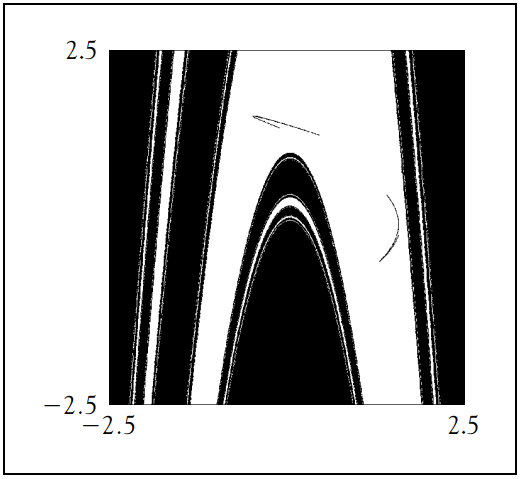
\includegraphics[width=.5\textwidth]{prob4.png}
			\end{figure}
			\item \textbf{Extra-Credit:} Use MatLab to create a colored heat map displaying the steady-state temperature distribution in this region. You  must include your program.
			\\ \\
			Let the following be true:
			\[u(r,\theta) = \phi(\theta)G(r)\]
			Notice the boundary conditions:
			\[\phi(\pi) = 0 \qquad \phi'(0) = 0 \qquad u(2,\theta) = \pi - \theta \]
			Taking Laplace's Equation, we get the following:
			\[\frac{r}{G}\frac{d}{dr}\left(r \frac{dG}{dr}\right) = -\frac{\phi''}{\phi} = \lambda\]
			From this, we get the following:
			\[\phi'' + \lambda\phi = 0 \qquad r\frac{d}{dr}\left(r \frac{dG}{dr}\right) - \lambda G = r^2G'' + rG' - \lambda G = 0\]
			\newpage
			From this, we can see this is an eigenvalue problem:
			\begin{enumerate}[label = (\alph*)]
				\item $(\lambda = 0)$:
				\[\phi'' = 0 \qqarrow \phi' = c_1 \qqarrow \phi = c_1 \theta + c_2\]
				\[r\frac{d}{dr}\left(r \frac{dG}{dr}\right) = 0 \qqarrow r \frac{dG}{dr} = d_1 \qqarrow G =  d_1\ln\,r + d_2 \]
				Substituting in our BC’s, we get:
				\[\phi'(0) = c_1 = 0 \qqarrow \phi(\pi) = c_2 = 0 \qqarrow \phi(\theta) = 0\]
				Thus we get the following trivial solution:
				\[\boldsymbol{u(r,\theta) = 0}\]
				\item $(\lambda < 0)$:
				\[\phi'' - |\lambda|\phi = 0\]
				Using the characteristic equation, we get:
				\[\phi(\theta) = c_1\cosh(\sqrt{|\lambda|}\theta) + c_2\sinh(\sqrt{|\lambda|}\theta) \qquad \phi'(\theta) = c_1\sqrt{|\lambda|}\sinh(\sqrt{|\lambda|}\theta) + c_2\sqrt{|\lambda|}\cosh(\sqrt{|\lambda|}\theta) \]
				Using the BC's, we get:
				\[\phi'(0) = c_2\sqrt{|\lambda|} = 0 \qqarrow c_2 = 0\]
				\[\phi(\pi) = c_1\cosh(\sqrt{|\lambda|}\pi) = 0 \qquad \cosh(\sqrt{|\lambda|}\pi) \not = 0 \qqarrow c_1 = 0 \]
				Thus we get the following trivial solution:
				\[\boldsymbol{u(r,\theta) = 0}\]
				\newpage
				\item $(\lambda > 0)$:
				\[\phi'' + \lambda\phi = 0\]
				Using the characteristic equation, we get:
				\[\phi(\theta) = c_1\cos(\sqrt{\lambda}\theta) + c_2\sin(\sqrt{\lambda}\theta) \qquad \phi'(\theta) = -c_1\sqrt{\lambda}\sin(\sqrt{\lambda}\theta) + c_2\sqrt{\lambda}\cos(\sqrt{\lambda}\theta)  \]
				Using the BC's, we get:
				\[\phi'(0) = c_2\sqrt{\lambda} = 0 \qqarrow c_2 = 0\]
				\[\phi(\pi) = c_1\cos(\sqrt{\lambda}\pi)\]
				\begin{enumerate}[label = (\roman*)]
					\item $(c_1 = 0)$:
					\[\phi(\theta) = 0\]
					Thus we get the following trivial solution:
					\[\boldsymbol{u(r,\theta) = 0}\]
					\item $(\cos(\sqrt{\lambda}\pi) = 0)$:
					\[\cos(\sqrt{\lambda}\pi) = 0 \qqarrow \sqrt{\lambda}\pi = \frac{(2n-1)\pi}{2} \qqarrow \lambda = \frac{(2n-1)^2}{4}\]
					So now we have our $n$ eigenfunctions:
					\[\phi_n(\theta) = c_1\cos\left(\frac{(2n-1)\theta}{2}\right) \]
					we can now substitute our eigenvalues into the other ODE, and we get:
					\[r^2G'' + rG' - \frac{(2n-1)^2}{4} G = 0\]
					Let the following be true:
					\[G = cr^\alpha \qqarrow G' = \alpha c r^{\alpha - 1} \qqarrow G'' = (\alpha^2 - \alpha) c r^{\alpha - 2}\]
					\begin{align*}
						r^2(\alpha^2 - \alpha)cr^{\alpha - 2} + r\alpha c r^{\alpha - 1} - \frac{(2n-1)^2}{4}cr^\alpha &= 0 \\
						r^{\alpha}c \left( \alpha^2 - \alpha  + \alpha  - \frac{(2n-1)^2}{4}\right) &= 0 \\
						\alpha &= \pm \frac{(2n-1)}{2}
					\end{align*}
					When solving this ODE, we get the following linear independent solutions:
					\[G(r) = d_1 r^{-\frac{(2n-1)}{2}} + d_2 r^{\frac{(2n-1)}{2}}\]
					Now we can solve for $G(r)$ using boundedness condition. This implies that $d_1 = 0$, thus we get:
					\[G_n(r) = d_2r^\frac{(2n-1)}{2}\]
					From here, we get the following $n$ product solutions:
					\[\boldsymbol{u_n(r,\theta) = A_nr^\frac{(2n-1)}{2}\cos\left(\frac{(2n-1)\theta}{2}\right) }\]
				\end{enumerate}
			\end{enumerate}
			\newpage
			By the Principle of Superposition, we get the following:
			\begin{align*}
				u(r,\theta) &= u_0(r,\theta) + u_1(r,\theta) + ... + u_n(r,\theta) \\
				&= \sum_{n=1}^{\infty} A_nr^\frac{(2n-1)}{2}\cos\left(\frac{(2n-1)\theta}{2}\right)
			\end{align*}
			We can now include our nonhomogeneous solution and get the following:
			\[u(2,\theta) = g(\theta) = \pi - \theta = \sum_{n=1}^{\infty} A_n(2)^\frac{(2n-1)}{2}\cos\left(\frac{(2n-1)\theta}{2}\right)\]
			Using the orthogonality of cosines, we get the following coefficients:
			\begin{align*}
				A_n &= \frac{2}{(2)^\frac{(2n-1)}{2}\pi}\int_{0}^{\pi}(\pi - \theta)\cos\left(\frac{(2n-1)\theta}{2}\right)\,d\theta \\
				&= \frac{2}{(2)^\frac{(2n-1)}{2}\pi}\left( (\pi - \theta)\left(\frac{2}{(2n-1)}\sin\frac{(2n-1)\theta}{2}\right) - \frac{4}{(2n-1)^2}\cos\frac{(2n-1)\theta}{2}\right)\bigg|_0^\pi  \\
				&= \frac{2^{3 - \frac{(2n-1)}{2}}}{(2n-1)^2\pi}
			\end{align*}
		\end{enumerate}
	\end{problem}

	\begin{problem}{5}
		If convection is taken into account, the equation for heat conduction and convection in a
		one-dimensional rod is given by:
		\[\pard{u}{t} = k\pard{^2u}{x^2} - v_0\pard{u}{x}, \qquad 0 < x < L, \qquad t > 0.\]
		Let $k = 1$, $v_0 = 0.6,$ and $L = 5.$ Assume the following boundary conditions and initial conditions:
		\[u(0,t) = 0, \quad u(L,t) = 0, \quad \text{ and } \quad u(x,0) = f(x)\]
		\begin{enumerate}[label = (\alph*)]
			\item Use separation of variables to create two ordinary differential equations
			\\ \\
			First we can rewrite the given equation:
			\[\pard{u}{t} = \pard{^2u}{x^2} - 0.6\pard{u}{x}, \qquad 0 < x < 5, \qquad t > 0.\]
			Let the following be true:
			\[u(x,t) = \phi(x)G(t) \qquad \phi(0) = 0, \quad \phi(5) = 0,\]
			Thus we get the following:
			\[\phi(x)G'(t) = \phi''(x)G(t) - 0.6\phi'(x)G(t)\]
			Now we can separate the equation to give us:
			\[\frac{G'}{G} = \frac{\phi''}{\phi} -0.6\frac{\phi'}{\phi} = -\lambda\]
			\item From the spatial ordinary differential equation, create a Sturm-Liouville eigenvalue problem.
			Identify explicitly the functions $p(x), q(x)$, and $\sigma(x)$. Find the eigenvalues and eigenfunctions
			for this problem. Explicitly write the orthogonality condition for this problem.
			\\ \\
			Notice the Sturm-Liouville eigenvalue problem form:
			\[\frac{d}{dx}\left[p(x)\frac{d\phi}{dx}\right] + [\lambda\sigma(x) + q(x)]\phi\]
			Notice the spatial ordinary differential equation:
			\[\phi'' -0.6\phi' + \lambda\phi = 0\]
			We can now multiply both sides by $e^{-0.6x}$ to give us:
			\[e^{-0.6x}\phi'' -0.6e^{-0.6x}\phi' + e^{-0.6x}\lambda\phi = 0\]
			Now we can rewrite this equation to put it in the form of the Sturm-Liouville eigenvalue problem:
			\[\frac{d}{dx}\left(e^{-0.6x}\phi'\right) + e^{-0.6x}\lambda\phi = 0 \]
			Thus we get the following:
			\[p(x) = e^{-0.6x} \qquad q(x) = 0 \qquad \sigma(x) = e^{-0.6x}\]
			Notice the Rayleigh Quotient:
			\[\lambda = \frac{-p(x)\phi(x)\phi'(x)\bigg|_a^b + \int_{a}^{b} \bigg[p(x)\left(\frac{d\phi}{dx}\right)^2 - q(x)\phi^2(x)\bigg]\,dx}{\int_{a}^b \phi^2(x)\sigma(x)\,dx}\]
			Substituting our parameters and using our BC's, we get:
			\begin{align*}
				\lambda &= \frac{-e^{-0.6x}\phi(x)\phi'(x)\bigg|_0^5 + \int_{0}^{5} \bigg[e^{-0.6x}\left(\frac{d\phi}{dx}\right)^2 \bigg]\,dx}{\int_{0}^5 \phi^2(x)e^{-0.6x}\,dx} \\
				&= \int_{0}^{5} \bigg[e^{-0.6x}\left(\frac{d\phi}{dx}\right)^2 \bigg]\,dx \bigg/ \int_{0}^5 \phi^2(x)e^{-0.6x}\,dx
			\end{align*}
			Notice that the Rayleigh Quotient tells us that the following has to be true: 
			\[\lambda > 0\] 
			Notice we the eigenvalues and eigenfunctions, from the following:
			\[\phi'' - 0.6\phi' + \lambda\phi = 0\]
			Using the characteristic equation, we get:
			\begin{enumerate}[label = (\alph*)]
				\item For ($0 < \lambda < 0.9$):
				\[\phi(x) = e^{0.3x}\left(c_1\cosh\left( (0.9 - \lambda)x \right) + c_2\sinh\left( (0.9 - \lambda)x \right) \right) \]
				Substituting our boundary conditions, gives us:
				\[\phi(0) = c_1 = 0 \qquad \phi(5) = c_2e^{1.5}\sinh\left(4.5 - 5\lambda \right) \qarrow c_2 = 0\]
				Thus, we get the trivial solution:
				\[\boldsymbol{\phi(x) = 0 \qqarrow u(x,t) = 0}\]
				\item For ($\lambda = 0.9$):
				\[\phi(x) = e^{0.3x}\left(c_1x + c_2\right) \]
				Substituting our boundary conditions, gives us:
				\[\phi(0) = c_2 = 0 \qquad \phi(5) = 5c_1e^{1.5} \qarrow c_1 = 0\]
				Thus, we get the trivial solution:
				\[\boldsymbol{\phi(x) = 0 \qqarrow u(x,t) = 0}\]
				\newpage
				\item For ($\lambda > 0.9$):
				\[\phi(x) = e^{0.3x}\left(c_1\cos\left( (\lambda - 0.9)x \right) + c_2\sin\left( (\lambda - 0.9)x\right)  \right) \]
				Substituting our boundary conditions, gives us:
				\[\phi(0) = c_1 = 0 \qquad \phi(5) = c_2e^{1.5}\sin(5\lambda - 4.5) \qquad 5\lambda - 4.5 = n\pi \qarrow \lambda_n = \frac{n\pi}{5} + 0.9\]
				So thus, we get the following eigenvalues and eigenfunctions:
				\[\boldsymbol{\lambda_n = \frac{n\pi}{5} + 0.9 \qqarrow \phi_n(x) = B_ne^{0.3x}\sin\left(\frac{n\pi x}{5}\right)}\]
				Notice the orthogonality condition:
				\[\int_{0}^5 e^{0.3x}\sin\left(\frac{m\pi x}{5}\right)\sin\left(\frac{n\pi x}{5}\right)\,dx  \]
			\end{enumerate}
			\item Solve the original partial differential equation with its boundary and initial conditions. Write
			clearly your integral for finding the Fourier coefficients.
			\\ \\
			Using our eigenvalues, we can solve for our time dependent equation:
			\[G' + \lambda G = 0 \qqarrow G' + \left(\frac{n\pi}{5} + 0.9\right)  G = 0 \qqarrow G = Ce^{-\left(\frac{n\pi}{5} + 0.9\right)t}\]
			Now we have our solution:
			\[\boldsymbol{u(x,t) = \sum_{n=1}^\infty B_ne^{0.3x}\sin\left(\frac{n\pi x}{5}\right)e^{-\left(\frac{n\pi}{5} + 0.9\right)t}}\]
			Using our initial condition, we get the following:
			\[u(x,0) = f(x) = \sum_{n=1}^\infty B_ne^{0.3x}\sin\left(\frac{n\pi x}{5}\right)\]
			with the following coefficient:
			\[\boldsymbol{B_n = \int_{0}^5 f(x)\sin\left(\frac{m\pi x}{5}\right) \bigg/ \int_{0}^5 e^{0.3x}\sin\left(\frac{n\pi x}{5}\right) \sin\left(\frac{m\pi x}{5}\right)}\]
		\end{enumerate}
	\end{problem}

	\begin{problem}{6}
		\begin{enumerate}[label = (\alph*)]
			\item The displacement of a uniform thin beam in a medium that resists motion satisfies the
			beam equation:
			\[\pard{^4}{x^4} = -\pard{^2u}{t^2} - 0.1\pard{u}{t}, \qquad 0 < x < 2, \qquad t > 0.\]
			If the beam is simply supported at the ends, then the boundary conditions are:
			\[u(0,t) = 0, \qquad u_{xx}(0,t) = 0, \qquad u(2,t) = 0, \qquad u_{xx}(2,t) = 0.\]
			Assume that there is initially no displacement and that an initial velocity, $u_t(x, 0) = 1$ is given
			to the beam. Solve this initial-boundary value problem. You can assume that the eigenvalues
			are real, but show clearly how you obtain all eigenvalues and eigenfunctions.
			\\ \\
			Let the following be true:
			\[u(x,t) = \phi(x)G(t)\]
			with the following conditions:
			\[\phi(0) = 0 \qquad \phi''(0) = 0 \qquad \phi(2) = 0 \qquad \phi''(2) = 0 \qquad G(0) = 0\]
			Using this information, we get the following:
			\[\phi^{(4)}(x)G(t) = - \phi(x)G''(t) - 0.1\phi(x)G'(t)\]
			We can separate this equation to get the following:
			\[-\frac{\phi^{(4)}}{\phi} = \frac{G''}{G} + 0.1\frac{G'}{G} = \lambda\]
			From this we get the following:
			\[\phi^{(4)} + \lambda\phi = 0 \qquad G'' + 0.1G' - \lambda G = 0\]
			\newpage
			From this, we can see this is an eigenvalue problem:
			\begin{enumerate}[label = (\alph*)]
				\item ($\lambda = 0$):
				\[\phi^{(4)} = 0 \quad \phi^{(3)} = c_1 \quad \phi'' = c_1x + c_2 \quad \phi' = \frac{c_1x^2}{2} + c_2x + c_3 \quad \phi = \frac{c_1x^3}{6} + \frac{c_2x^2}{2} + c_3x + c_4\]
				\[G'' + 0.1G' = 0 \qqarrow G = c_1e^{-0.1x} + c_2 \qquad G' = -0.1c_1e^{-0.1x} \qquad G'' = 0.01c_1e^{-0.1x}\]
				Substituting in our BC's, we get:
				\[\phi(0) = 0 = c_4 \qquad \phi''(0) = 0 = c_2 \qquad \phi(2) = 0 = \frac{4c_1}{3} + 2c_3 \qquad \phi''(2) = 0 = 2c_1\]
				Thus, we can see that $c_1 = c_2 = c_3 = c_4 = 0, \quad\Longrightarrow\quad \phi = 0$, and get the following trivial solution:
				\[\boldsymbol{u(x,t) = 0}\]
				\item ($\lambda < 0$):
				\[\phi^{(4)} - |\lambda|\phi = 0\]
				Using the characteristic equation, we get:
				\[\phi(x) = c_1\cosh(\sqrt[4]{|\lambda|}x)+ c_2\sinh(\sqrt[4]{|\lambda|}x) \qquad \phi''(x) = c_1\sqrt{|\lambda|}\cosh(\sqrt[4]{|\lambda|}x)+ c_2\sqrt{|\lambda|}\sinh(\sqrt[4]{|\lambda|}x)\]
				Using the BC's, we get:
				\[\phi(0) = 0 = c_1 \qquad \phi(2) = 0 = c_2\sinh(2\sqrt[4]{|\lambda|}) \qarrow c_2 = 0\]
				Thus, we get the following trivial solution:
				\[\boldsymbol{u(x,t) = 0}\]
				\item ($\lambda > 0$):
				\[\phi^{(4)} + \lambda\phi = 0\]
				Using the characteristic equation, we get:
				\[\phi(x) = c_1\cos(\sqrt[4]{\lambda}x)+ c_2\sin(\sqrt[4]{\lambda}x) \qquad \phi''(x) = -c_1\sqrt{\lambda}\cos(\sqrt[4]{\lambda}x)- c_2\sqrt{\lambda}\sin(\sqrt[4]{\lambda}x)\]
				Using the BC's, we get:
				\[\phi(0) = 0 = c_1 \qquad \phi(2) = 0 = c_2\sin(2\sqrt[4]{\lambda}) \qquad \phi''(2) = -c_2\sqrt{\lambda}\sin(2\sqrt[4]{\lambda})\]
				If we let $c_2 = 0$, we get the following trivial solution:
				\[u(x,t) = 0\]
				If we let $\sin(2\sqrt[4]{\lambda}) = 0$, we get the following $n$ eigenvalues:
				\[\sin(2\sqrt[4]{\lambda_n}) = 0 \qqarrow 2\sqrt[4]{\lambda_n} = n\pi \qqarrow \lambda_n = \left( \frac{n\pi}{2}\right)^4\]
				So now we get the following $n$ eigenfunctions:
				\[\phi_n(x) = c_2\sin\left( \frac{n\pi x}{2}\right) \]
				We can now substitute our eigenvalues into the other ODE, and we get:
				\[G'' + 0.1G' - \left( \frac{n\pi}{2}\right)^4G = 0\]
				Using the characteristic equation, we get the following solution:
				\[G(t) = e^{-0.05t}\left( c_1\cosh\left(\frac{\sqrt{0.01+\frac{(n\pi)^4}{4}}}{2}t\right) + c_2\sinh\left(\frac{\sqrt{0.01+\frac{(n\pi)^4}{4}}}{2}t\right) \right) \]
				Using the BC's, we get:
				\[G(0) = 0 = c_1 \qqarrow c_1 = 0\]
				Thus we get the following:
				\[G_n(t) = c_2e^{-0.05t}\sinh\left(\frac{\sqrt{0.01+\frac{(n\pi)^4}{4}}}{2}t\right)\]
				From here, we get the following $n$ product solutions:
				\[u_n(x,t) = B_ne^{-0.05t} \sinh\left(\frac{\sqrt{0.01+\frac{(n\pi)^4}{4}}}{2}t\right)\sin\left( \frac{n\pi x}{2}\right)\]
			\end{enumerate}
			By the Principle of Superposition, we get the following:
			\begin{align*}
				\boldsymbol{u(x,y)} &= u_0(x,y) + u_1(x,y) + ... + u_n(x,y) \\
				&= \boldsymbol{\sum_{n=1}^{\infty} B_ne^{-0.05t} \sinh\left(\frac{\sqrt{0.01+\frac{(n\pi)^4}{4}}}{2}t\right)\sin\left( \frac{n\pi x}{2}\right)}
			\end{align*}
			Notice the derivative of $u$ in respect to $t$:
			\[\pard{u}{t} = \sum_{n=1}^{\infty} B_n\left( \frac{\sqrt{0.01+\frac{(n\pi)^4}{4}}}{2\,e^{0.05t}} \cosh\left(\frac{\sqrt{0.01+\frac{(n\pi)^4}{4}}}{2}t\right) - 0.05e^{-0.05t} \sinh\left(\frac{\sqrt{0.01+\frac{(n\pi)^4}{4}}}{2}t\right)\right) \sin\left( \frac{n\pi x}{2}\right)\]
			We can now include our nonhomogeneous solution and get the following:
			\[\pard{u}{t}(x,0) = 1 = \sum_{n=1}^{\infty} B_n\frac{\sqrt{0.01+\frac{(n\pi)^4}{4}}}{2} \sin\left( \frac{n\pi x}{2}\right)\]
			Using the orthogonality of sines, we get:
			\[\boldsymbol{B_n = \frac{2}{\sqrt{0.01+\frac{(n\pi)^4}{4}}}\int_{0}^2 \sin\left( \frac{n\pi x}{2}\right)\,dx =  \frac{-4\left((-1)^n - 1\right)}{n\pi\sqrt{0.01+\frac{(n\pi)^4}{4}}}}\]
			\newpage
			\item Use 20 terms in the series solution of $u(x, t)$ and have the computer graph the displacement
			of the beam at times $t = 0, 1, 2, 5, 10$, and $20$.
			\lstinputlisting[language=Matlab]{./Code/Prob6b.m}
			\begin{figure}[h!]
				\centering
				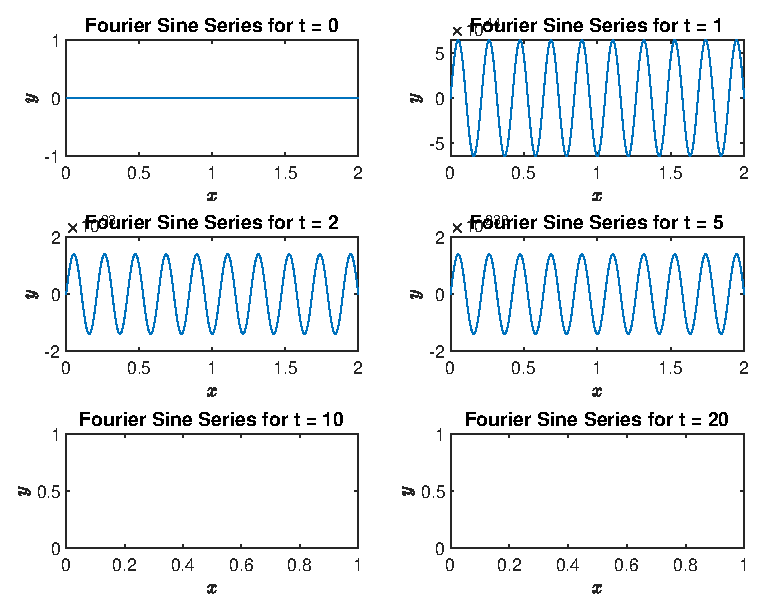
\includegraphics[width=.6\linewidth]{./Code/Prob6b}
			\end{figure}
			\skipline
			Notice for $t = 10, t = 20$, the values are out of range for Matlab.
			\item
\textbf{Extra-Credit:} Use MatLab to create a smooth surface showing the time evolution of the
			beam for $0 \leq x \leq 2$ and $0 \leq t \leq 50$. You must include your program.
		\end{enumerate}
		
	\end{problem}


\end{document}
